\documentclass{article}

\usepackage{fullpage}
\usepackage{color}
\usepackage{amsmath}
\usepackage{url}
\usepackage{verbatim}
\usepackage{graphicx}
\usepackage{parskip}
\usepackage{amssymb}
\usepackage{nicefrac}
\usepackage{listings} % For displaying code
\usepackage{algorithm2e} % pseudo-code

% Answers
\def\ans#1{\par\gre{Answer: #1}}
%\def\ans#1{} % Comment this line to produce document with answers

% Colors
\definecolor{blu}{rgb}{0,0,1}
\def\blu#1{{\color{blu}#1}}
\definecolor{gre}{rgb}{0,.5,0}
\def\gre#1{{\color{gre}#1}}
\definecolor{red}{rgb}{1,0,0}
\def\red#1{{\color{red}#1}}
\def\norm#1{\|#1\|}

% Math
\def\R{\mathbb{R}}
\def\argmax{\mathop{\rm arg\,max}}
\def\argmin{\mathop{\rm arg\,min}}
\newcommand{\mat}[1]{\begin{bmatrix}#1\end{bmatrix}}
\newcommand{\alignStar}[1]{\begin{align*}#1\end{align*}}

% LaTeX
\newcommand{\fig}[2]{\includegraphics[width=#1\textwidth]{a1f/#2}}
\newcommand{\centerfig}[2]{\begin{center}\includegraphics[width=#1\textwidth]{a1f/#2}\end{center}}
\def\items#1{\begin{itemize}#1\end{itemize}}
\def\enum#1{\begin{enumerate}#1\end{enumerate}}
\newcommand{\matCode}[1]{\lstinputlisting[language=Matlab]{a1f/#1.m}}


\begin{document}

\title{CPSC 340 Assignment 1 (due Friday September 29 ATE)}
\author{}
\date{}
\maketitle
\vspace{-4em}


Name: Hang Yee Wong\\
CS ID: r9i0b

Name: Joanne Chen\\
CS ID: r0a9


\section{Summary Statistics and Data Visualization}

\subsection{Summary Statistics}

\begin{verbatim}

minimum(X) =  0.352

maximum(X) = 4.862

mean(X) = 1.3246249999999997

median(X) = 1.1589999999999998

mode(X) = 0.77

\end{verbatim}

The mode isn't very reliable because a lot of these data points have the same integer values but different decimal values. To give a meaningful mode, we can make the data discrete by rounding the data points.



\subsection{Data Visualization}

\begin{enumerate}
\item C
\item B
\item F
\item D
\item E
\item A
\end{enumerate}


\subsection{Decision Surfaces}

There are 9 green crosses on the side classified to be blue and 8 blue circles on the green side, so a total of 17 examples were mis-classified.

\section{Decision Trees}


\subsection{Equality vs. Inequality Splitting Rules}

It might make more sense when working with features with few, discrete values that are not related. For example, with "colour" as a feature converted to numbers, inequalities wouldn't make a lot of sense as the numbers representing the colours are not related in quantity.

\subsection{Decision Stump Implementation}
\begin{verbatim}
function decisionStump(X,y)
    # Get the size of the data matrix
    (n,d) = size(X)

    # Initial the best rule with the baseline rule (no split)
    y_mode = mode(y)
    minError = sum(y .!= y_mode);
    splitVariable = [];
    splitValue = [];
    splitYes = y_mode;
    splitNo = [];

    # Search for the best rule
    # (Uses O(n^2d) approach to keep code simple)
    yhat = zeros(n)
    for j in 1:d
        # Try unique values of column as split values
        for val in unique(X[:,j])

            # Test whether each object satisfies equality
            yes = X[:,j] .> val

            # Find correct label on both sides of split
            y_yes = mode(y[yes])
            y_no = mode(y[.!yes])

            # Make predictions
            yhat[yes] = y_yes
            yhat[.!yes] = y_no

            # Compute error
            trainError = sum(yhat .!= y)

            # Update best rule
            if trainError < minError
	            minError = trainError
                splitVariable = j
                splitValue = val
                splitYes = y_yes
                splitNo = y_no
            end
        end
    end

    # Now that we have the best rule,
    # let's build our splitting function
    function split(Xhat)
        (t,d) = size(Xhat)
        if isempty(splitVariable)
            return fill(true,t)
        else
		    return (Xhat[:,splitVariable] .> splitValue)
        end
    end

    # Now that we have the best rule,
    # let's build our predict function
    function predict(Xhat)
        (t,d) = size(Xhat)
        yes = split(Xhat)
        yhat = fill(splitYes,t)
        if any(.!yes)
            yhat[.!yes] = splitNo
        end
        return yhat
    end

    return StumpModel(predict,split,isempty(splitNo))
end
\end{verbatim}

Code can also be found in \texttt{decisionStump.jl}\\
Training Error of \texttt{decisionStump}: 0.25

\subsection{Constructing Decision Trees}
\begin{verbatim}
if latitude > 37.669007
    if longitude > -96.090109
        return 1
    else
        return 2
else
    if longitude > -115.577574
        return 2
    else
        return 1
\end{verbatim}



\subsection{Cost of Fitting Decision Trees}

The first (top-level) decision stump takes $O(nd\log{n})$ time, and as we split, the second-level decision stumps each takes $O(nd\log{\frac{n}{a}})$ and $O(nd\log{\frac{n}{b}})$ time, where $\frac{n}{a} + \frac{n}{b} = n$. So the second layer takes $O(nd\log{n})$ time still. We apply the same reasoning to each layer, and we have a total of $m$ layers, so the total cost is $O(mnd\log{n})$ time.

\section{Training and Testing}

\subsection{Training Error}

Initially, the training error of \texttt{decisionStump} decreases as the depth increases, but it stops decreasing after depth 4. On the other hand, the training error of infogain decreases with increasing depth all the way to zero.

The error stops decreasing after a certain depth for the decision tree model likely because the splitting isn't even and sometimes the NO case has no more objects even when there are still objects of different labels in the same YES case. When this happens, we have reached the base split case and our implementation of \texttt{decisionTree} will split no further, meaning that some of the objects that end up in the same YES-leaf have different labels, which means some of them will be assigned labels different from the actual labels they have, which increases the training error regardless of what value is assigned to them.

\subsection{Training and Testing Error Curves}

\textit{
Legend:
\begin{itemize}
	\item blue crosses are training errors
	\item red dots are test errors
	\item x-axis represents the depth
	\item y-axis represents the error
\end{itemize}}

\begin{figure}[h!]
  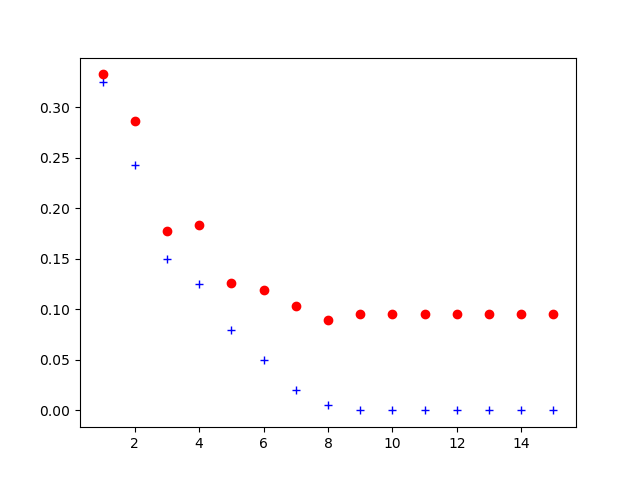
\includegraphics[height=7.5cm]{Etrain_Etest_vs_depth.png}
  \caption{Training Error and Test Error vs. Depth}
  \label{fig: error vs depth}
\end{figure}


\subsection{Validation Set}

If we split the dataset in half and use the first half for training and second half for validation, the minimum validation set error we were able to obtain was 0.165 at depth 4 with a 0.110 train error, but after depth 4 the validation set error stays the same. If we switch the data sets and use the second half for training and first half for validation, the minimum validation error becomes 0.155 at depth 4 with a 0.105 training error. To use more of our data to estimate depth, we could use cross validation so every object is used for validation once.

\section{Naive Bayes}

In this section we'll implement naive Bayes, a very fast classification method that is often surprisingly accurate for text data with simple representations like bag of words.



\subsection{Naive Bayes by Hand}

(a)
\begin{enumerate}
\item  $\frac{6}{10}$
\item  $\frac{4}{10}$
\end{enumerate}

(b)
\begin{enumerate}
\item  $\frac{1}{2}$
\item  $\frac{1}{3}$
\item  $1$
\item  $\frac{3}{4}$
\end{enumerate}

(c)\\
$p( y = 1 |  x_1 = 1 , x_2 = 0 )
    \\ \propto p(  x_1 = 1  | y = 1 ) p(  x_2 = 0  | y = 1 ) p( y =1)$.
    \newline = $ (\frac{1}{2}) (\frac{1}{3})(\frac{6}{10}) $
    \newline = $0.1$
\\\\
$p( y = 0 |  x_1 = 1 , x_2 = 0 )
        \\\propto p(  x_1 = 1  | y = 0 ) p(  x_2 = 0  | y = 0 ) p( y =0)$.
        \newline =$ (1) (\frac{3}{4})(\frac{4}{10}) $
        \newline = $0.3$
\newline
\\Since the $p( y = 0 |  x_1 = 1 , x_2 = 0 ) $ is bigger , the most likely label is 0.


\subsection{Bag of Words}

\begin{enumerate}
\item  $"league"$
\item  $"car", "engine", "evidence", "problem", "system"$
\item $"rec.*"$

\end{enumerate}


\subsection{Naive Bayes Implementation}
\begin{verbatim}
    function naiveBayes(X,y)
    # Implementation of naive Bayes classifier for binary features

    (n,d) = size(X)

    # Compute number of classes, assuming y in {1,2,...,k}
    k = maximum(y)

    # We will store p(y(i) = c) in p_y(c)
    counts = zeros(k)
    for i in 1:n
      counts[y[i]] += 1
    end
    p_y = counts ./= n

    # We will store p(x(i,j) = 1 | y(i) = c) in p_xy(1,j,c)
    # We will store p(x(i,j) = 0 | y(i) = c) in p_xy(2,j,c)

    p_xy = zeros(2,d,k)

    # Q4.3
    function cal_p_xy(X, j, c, xval)
      (n,d) = size(X)
      match = 0;
      total = 0
      Xj = X[:,j]
      for a in 1:n

        if (y[a] == c)
          total += 1
          if (Xj[a] == xval)
            match += 1
          end
        end

      end

      return (total == 0) ? 0 : match / total
    end

    for c in 1:k
      for j in 1:d
        p_xy[1,j,c] = cal_p_xy(X,j,c,1)
        p_xy[2,j,c] = cal_p_xy(X,j,c,0)
      end
    end

    function predict(Xhat)
      (t,d) = size(Xhat)
      yhat = zeros(t)

      for i in 1:t
        # p_yx = p_y*prod(p_xy) for the appropriate x and y values
        p_yx = copy(p_y)
        for j in 1:d
          if Xhat[i,j] == 1
            for c in 1:k
              p_yx[c] *= p_xy[1,j,c]
            end
          else
            for c in 1:k
              p_yx[c] *= p_xy[2,j,c]
            end
          end
          (~,yhat[i]) = findmax(p_yx)
        end
      end
      return yhat
    end

    return GenericModel(predict)
  end
\end{verbatim}


Code can also be found in \texttt{naiveBayes.jl}

\subsection{Runtime of Naive Bayes for Discrete Data}

The cost of classifying is $O(tdk)$. Because the dominant cost is computing $p(X_{ij} | Y_{i})$. And we have it with three for loops: loop over the examples $t$, and loop over the features $d$, and loop over the class labels $k$.


\section{K-Nearest Neighbours}

\subsection{KNN Prediction}

\begin{enumerate}
    \item Code can also be found in \texttt{knn.jl} \\
    \begin{verbatim}
        function knn_predict(Xhat,X,y,k)
            (n,d) = size(X)
            (t,d) = size(Xhat)
            k = min(n,k) # To save you some debuggin

            D = zeros(t, n)
            yhat = zeros(t)

            for i in 1:t
                for j in 1:n
                    D[i, j] = sqrt(sum((Xhat[i,:] .- X[j,:]).^2))
                end
            end

            for i in 1:t
                rank = sortperm(D[i,:])
                yhat[i] = mode(y[rank[1:k]])
            end

            return yhat
        end
    \end{verbatim}
	\item $x(k, Etrain, Etest) = (1, 0.000, 0.286), (3, 0.028, 0.286), (10, 0.072, 0.286)$
	\item See Figure 2 below
	\item This is because the there is only one nearest neighbour and the nearest neighbour of any point in \texttt{Xhat} is always itself as \texttt{Xhat} is equal to \texttt{X} when calculating the training error. This means the predicted label is always the same as the actual label, meaning the training error = 0.
	\item Use cross validation to choose the best $k$. Using the \texttt{citiesSmall} dataset a fold of 5 would probably make sense.
\end{enumerate}
\begin{figure}[h!]
  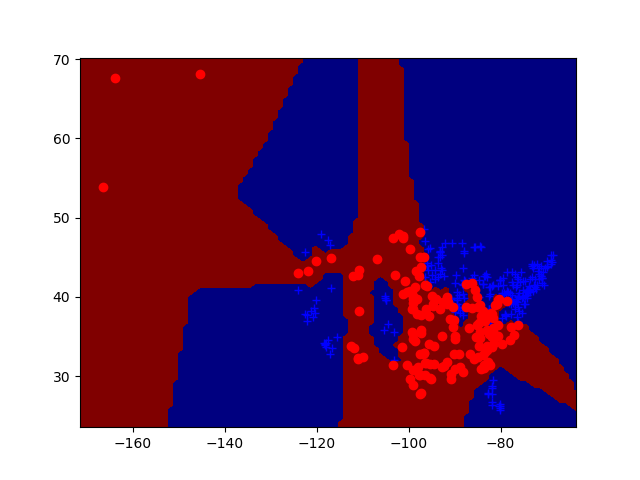
\includegraphics[height=7.5cm]{knn_train_data_k=1.png}
  \caption{KNN Training Data on k=1}
  \label{fig: knn}
\end{figure}

\subsection{Condensed Nearest Neighbours}

\enum{
	\item After training \texttt{cknn} on \texttt{X} of \texttt{citiesBig1}, running \texttt{predict} on \texttt{Xtest} of \texttt{citiesBig1} with $k = 1$ took 4.136411572 seconds. Running the same data using \texttt{knn} with the same $k$ took 140.647040979 seconds.
	\item Size of the subset = 457, $Etrain$ = 0.008, $Etest$ = 0.018
	\item This is because an object in the training data set might not be in the model anymore, so the nearest neighbour of an object might not always be itself, meaning the predicted label might not always match the actual label.
	\item We need to calculate the distance between each object in \texttt{Xhat} and each object in \texttt{Xsub}, so we need to calculate $ts$ distances in total. Each distance is calculated from $d$ dimensions, so the total cost is $O(tsd)$.
    \item $(k, Etrain, Etest) = (1, 0.138, 0.210), (3, 0.285, 0.227), (10, 0.571, 0.512)$. The high errors are likely due to the fact that the data set is sorted. This does not matter in \texttt{knn} as we use all the data points in \texttt{knn}. This will however influence the subset we choose in \texttt{cknn} as we decide whether or not to add a data point to the subset by looking at the previous data points. This means what we use to train the model is affected by all the data points before the current data point. In this case, \textit{citiesBig2} is likely to have the data points sorted in such a way that the outliers are added to the subset, resulting in high errors.
}

\section{Very-Short Answer Questions}

\begin{enumerate}
\item  Scatterplot could provide a brief idea of that data. For example, it could help us choose a better k in knn and a better depth in decision trees.
\item  If a data set is not chosen randomly, it is not IID. For example, some data points might be sampled much closer in time than other data points.
\item Validation set is a part of our training data used to approximate test error. Test set is for evaluation of the model and to provide the true test error, and we cannot access it during training.
\item Naive Bayes classifier assumes that the presence of a particular feature in a class is unrelated to the presence of any other feature.
\item The features of data are not independent of each other. For example, in bag of words, words that represent postal codes, addresses, and cities have a higher chance of appearing together than other words.
\item Non-parametric models don't grow with the size of the data set, so they tend to be a lot faster than parametric models when working with huge data sets.
\item It will not affect the training error as the relation between the data points would stay the same (i.e. distance in between the points would be proportional to before processing). However, this will affect the test error as the mean and variance of the test dataset is different. For example, a point that would have been above the threshold of a decision stump may now be below the threshold.
\item It will not affect the training and prediction. In the traing phrase, KNN always stores all the data in the model, regardless of what k is. In the prediction phase, KNN always computes all the distances between a point and all the other points, so k really only changes the runtime when we are taking the mode of the k nearest neighbours in the prediction phase, but because k is a constant and is typically much smaller than n and d, it will not affect the overall runtime asymptotically.
\item Training error increases as k increases (training error is 0 when k = 1). The approximation error decreases with k up to a certain threshold, then starts increasing after the threshold as it starts to take outliers into account.
\item For large n, the training error would increase and the approximation error would decrease because the model would become more general as n increases.
\end{enumerate}


\end{document}
